%%
%%############################
\newcommand{\prexo}{\emph{pre\_exodus \,}}
\newcommand{\bc}{\emph{bc-file \,}}
\newcommand{\head}{\emph{header-file \,}}

\chapter{FSI Tutorial 2d with \prexo and Cubit}
\label{tut_fsi_preexo:chap}

%%
%%============================
\section{Introduction}

As example, we consider a 2d driven cavity example as
sketched in Fig. \ref{tut_fsi_preexo_2d:1.1}.
Hint: In case you want or need to see a sample solution for this tutorial 
you will find corresponding files in the \baci{} subfolder \emph{/tests/framework-tests/}!
However, it is highly recommended to look at these files only in case you encounter severe problems
while stepping through the tutorial.\\
For further details and references we refer the reader to:\\
W.A. Wall, PhD thesis, 1999
(available under \texttt{/lnm/literature/1999/})

\begin{figure}[h]
\hfil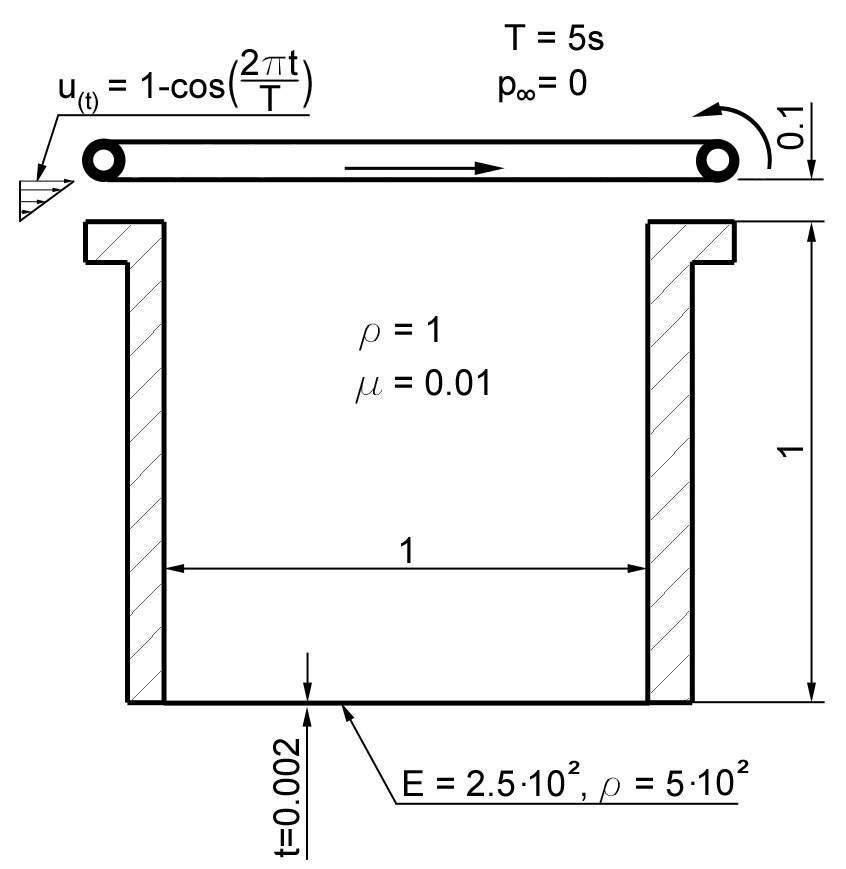
\includegraphics[scale=0.2]{Bilder/Angabeskizze}

\caption{\label{tut_fsi_preexo_2d:1.1} The driven cavity example in 2d}
\end{figure}

\section{Creating the Geometry with Cubit}

Besides meshing cubit also has several geometry creation methods. We refer
to the provided manual and tutorials. It supports scripting (also Python),
therefore we provide a \textit{Journal}-file containing the
necessary geometry commands as well as mesh and definitions for elements and
boundary conditions, respectively.

You can find this jpurnal file within you \baci{} distribution. It is located in
\textit{baci/tests/framework-test/tutorial\_fsi.jou}.


Within Cubit, open the Journal-Editor (\emph{Tools}$\to$\emph{Journal
Editor}), paste the text from the journal file and press \emph{play}. For later
usage it is convenient to save the current content of the Journal-Editor into a \emph{*.jou} file. 
Export now the created geometry and mesh to an
exodus-file (filename: dc2d.exo) via \emph{File}$\to$\emph{Export...}. 
During export, set the dimension explicitly to 2d.

\section{Working with \prexo and \baci{}}

\prexo is a C++ code embedded into the \baci{} environment. It is meant to
transfer a given mesh into a \baci{}-readable input file.

\subsection{Preliminaries}

If not already done, compile \prexo via \begin{verbatim}make pre_exodus\end{verbatim} after 
configuring \baci{} in the usual way.

\subsection{General Procedure of Creating a Valid \baci{} Input File}
With a given mesh including some nodal clouds to apply conditions to you need
another text-file (\bc) where you specify, what you would like to do with
it. It contains for example the specific element declaration (fluid, structure,
parameters, etc.) and the particular boundary condition such as Dirichlet or
Neumann. Finally, a \head consists of general parameters such as
solvers, algorithmic parameters, etc. Those three files are merged by \prexo
into an input file for \baci{}. This file is then \emph{automatically} validated
using all available \baci{} validation and is therefore likely to run.

Sure, you usually do not have already a proper \head and matching \bc. By
typing
\begin{center}
  \verb|./pre_exodus --exo=yourmesh.e|
\end{center}
you get two preliminary files
'default.head' and 'default.bc'. The first contains the currently valid header
parameters with default values and commented options which you can edit to
adapt it to your means. Similarly, 'default.bc' consists of all your mesh
entities and a list of all currently valid conditions. See next section for
details how to work with it and how to get valid input files.

\subsection{Running a Simulation with \baci{}}
\label{tut_fsi_preexo_2d:baci}
To start the solver use the call 
\begin{center}
	\verb|./baci-release [inputdirectory]/your_example.dat [outputdirectory]/outputprefix|
\end{center}
(in the \baci{}-directory). The results are then written to
the result directory with the prefix you chose.

\section{The FSI problem with a partitioned solver}
Here, we create the \baci{} input file for the FSI problem, that is solved using
partitioned scheme. For a monolithic scheme, see
section\ref{tut_fsi_preexo_2d:monolithic}.

Edit 'default.head' and 'default.bc'.

\subsection{\head}
Find the following sections in 'default.head' and edit as given:
\begin{itemize}

 \item \verb|ALE DYNAMIC|

 \verb|LINEAR_SOLVER        1|

 \item \verb|FLUID DYNAMIC|

 \verb|CONVTOL              1e-08|
 
 \verb|GRIDVEL              BDF2|
 
 \verb|ITEMAX               50|
 
 \verb|LINEAR_SOLVER        2|
 
 \verb|TIMEINTEGR           Np_Gen_Alpha|
 
 \item \verb|FSI DYNAMIC|

 \verb|MAXTIME              3|
 
 \verb|NUMSTEP              30|
 
 \verb|SECONDORDER          yes|

 \verb|SHAPEDERIVATIVES     yes|
 
 \verb|TIMESTEP             0.1|

 \item \verb|SOLVER 1|
 
 \verb|NAME                 ALE solver|

 \verb|SOLVER               UMFPACK|

 \item \verb|SOLVER 2|
 
 \verb|NAME                 Fluid solver|

 \verb|SOLVER               Aztec_MSR|

 \item \verb|SOLVER 3|
 
 \verb|NAME                 Structure solver|

 \verb|SOLVER               UMFPACK|

 \item \verb|STRUCTURAL DYNAMIC|

 \verb|LINEAR_SOLVER        3|
 
 \verb|TOLRES               1e-10|

 \item \verb|MATERIALS|
 
 insert \verb|MAT 1 MAT_fluid DYNVISCOSITY 0.01 DENSITY 1.0| for definition of
 fluid material
 
 insert \verb|MAT 2 MAT_ElastHyper NUMMAT 1 MATIDS 3 DENS 500| to define a
 hyperelastic structural material

 insert \verb|MAT 3 ELAST_CoupNeoHooke YOUNG 250.0 NUE 0.0| to specify the
 structural material as Neo-Hooke material
 
 insert \verb|MAT 4 MAT_Struct_StVenantKirchhoff YOUNG 1.0 NUE 0.0 DENS 1.0| to
 define an ALE material

 \item \verb|CLONING MATERIAL MAP|

 insert \verb|SRC_FIELD fluid SRC_MAT 1 TAR_FIELD ale TAR_MAT 4| to specify the
 ALE material that is used for the fluid field 

 \item \verb|CURVE 1|

 insert \verb|CURVE 1 on EXPR FUNC (1-cos(2*t*pi/5)) t1 0.0 t2 200.0| defining
time-dependent inflow and lid movement
 
  \item \verb|FUNCT 1|

 insert \verb|FUNCT 1 EXPR 0 0 0 FUNCTION 10*(y-1)| representing the spatial
 inflow distribution

\end{itemize}
Safe the file under a different name, e.g. 'dc2d\_fsi.head'.

\subsection{\bc}
Edit the 'default.bc' file as follows:

For the element definitions:

\begin{itemize}
  \item \verb|*eb1="ELEMENT"| \qquad the structure elements with their material
  \begin{small} \begin{verbatim}
      sectionname="STRUCTURE"
      description="MAT 2 KINEM nonlinear EAS none THICK 1.0 STRESS_STRAIN plane_strain GP 2 2"
      elementname="WALL"
    \end{verbatim} 
  \end{small}
 
 \item \verb|*eb2="ELEMENT"| \qquad the fluid elements with ALE and the
 fluid material
 \begin{small} \begin{verbatim}
      sectionname="FLUID"
      description="MAT 1 NA ALE"
      elementname="FLUID"
    \end{verbatim} 
  \end{small}
\end{itemize}

For Dirichlet boundary conditions for structure, fluid and ALE:

\begin{itemize}

  \item \verb|*ns1="CONDITION"| \qquad Fixing the structure at left and right
  side
  \begin{small} \begin{verbatim}
      sectionname="DESIGN LINE DIRICH CONDITIONS"
      description="NUMDOF 2 ONOFF 1 1 VAL 0.0 0.0 CURVE none none FUNCT 0 0"
    \end{verbatim} 
  \end{small}
  
  \item \verb|*ns2="CONDITION"| \qquad
  \begin{small} \begin{verbatim}
      sectionname="DESIGN FSI COUPLING LINE CONDITIONS"
      description="1"
    \end{verbatim}
   \end{small}
   
  \item \verb|*ns3="CONDITION"| \qquad
  \begin{small} \begin{verbatim}
      sectionname="DESIGN POINT DIRICH CONDITIONS"
      description="NUMDOF 2 ONOFF 1 1 VAL 0.0 0.0 CURVE none none FUNCT 0 0"
    \end{verbatim}
   \end{small}
   
  \item \verb|*ns4="CONDITION"| \qquad
  \begin{small} \begin{verbatim}
      sectionname="DESIGN POINT DIRICH CONDITIONS"
      description="NUMDOF 2 ONOFF 1 1 VAL 0.0 0.0 CURVE none none FUNCT 0 0"
    \end{verbatim}
   \end{small}
   
  \item \verb|*ns5="CONDITION"| \qquad
  \begin{small} \begin{verbatim}
      sectionname="DESIGN LINE DIRICH CONDITIONS"
      description="NUMDOF 3 ONOFF 1 1 0 VAL 0.0 0.0 0.0 CURVE none none none FUNCT 0 0 0"
    \end{verbatim}
   \end{small}
   
  \item \verb|*ns6="CONDITION"| \qquad
  \begin{small} \begin{verbatim}
      sectionname="DESIGN LINE DIRICH CONDITIONS"
      description="NUMDOF 3 ONOFF 1 1 0 VAL 1.0 0.0 0.0 CURVE 1 none none FUNCT 0 0 0"
    \end{verbatim}
   \end{small}
   
  \item \verb|*ns7="CONDITION"| \qquad
  \begin{small} \begin{verbatim}
      sectionname="DESIGN LINE DIRICH CONDITIONS"
      description="NUMDOF 3 ONOFF 1 1 0 VAL 1.0 0.0 0.0 CURVE 1 none none FUNCT 1 0 0"
    \end{verbatim}
   \end{small}
   
  \item \verb|*ns8="CONDITION"| \qquad
  \begin{small} \begin{verbatim}
      sectionname="DESIGN LINE ALE DIRICH CONDITIONS"
      description="NUMDOF 2 ONOFF 1 1 VAL 0.0 0.0 CURVE none none FUNCT 0 0"
    \end{verbatim}
   \end{small}
   
  \item \verb|*ns9="CONDITION"| \qquad
  \begin{small} \begin{verbatim}
      sectionname="DESIGN FSI COUPLING LINE CONDITIONS"
      description="1"
    \end{verbatim}
   \end{small}
   
  \item \verb|*ns10="CONDITION"| \qquad
  \begin{small} \begin{verbatim}
      sectionname="DESIGN POINT DIRICH CONDITIONS"
      description="NUMDOF 3 ONOFF 1 1 0 VAL 1.0 0.0 0.0 CURVE 1 none none FUNCT 0 0 0"
    \end{verbatim}
   \end{small}
   
  \item \verb|*ns11="CONDITION"| \qquad
  \begin{small} \begin{verbatim}
      sectionname="DESIGN POINT DIRICH CONDITIONS"
      description="NUMDOF 3 ONOFF 1 1 0 VAL 0.0 0.0 0.0 CURVE none none none FUNCT 0 0 0"
    \end{verbatim}
   \end{small}

  \item \verb|*ns12="CONDITION"| \qquad
  \begin{small} \begin{verbatim}
      sectionname="DESIGN POINT DIRICH CONDITIONS"
      description="NUMDOF 3 ONOFF 1 1 0 VAL 0.0 0.0 0.0 CURVE none none none FUNCT 0 0 0"
    \end{verbatim}
   \end{small}

  \item \verb|*ns13="CONDITION"| \qquad
  \begin{small} \begin{verbatim}
      sectionname="DESIGN POINT ALE DIRICH CONDITIONS"
      description="NUMDOF 2 ONOFF 1 1 VAL 0.0 0.0 CURVE none none FUNCT 0 0"
    \end{verbatim}
   \end{small}
\end{itemize}
   
Copy the following condition and parametrize it as given below to further
prescibe Dirichlet boundary conditions on the ALE field:
   
\begin{itemize}
  \item \verb|*ns6="CONDITION"| \qquad
  \begin{small} \begin{verbatim}
      sectionname="DESIGN LINE ALE DIRICH CONDITIONS"
      description="NUMDOF 2 ONOFF 1 1 VAL 0.0 0.0 CURVE none none FUNCT 0 0"
    \end{verbatim}
   \end{small}
\end{itemize}   

As any of these conditions matches an already defined NodeSet it will also match
the corresponding 'E-id' in the later \baci{} input file.
Finally save the file under a different name, e.g. 'dc2d\_fsi.bc'.

\subsection{Creating \baci{} Input File and Running the Simulation}
Run in a shell \begin{verbatim} ./pre_exodus --exo=dc2d.e --head=dc2d_fsi.head
--bc=dc2d_fsi.bc --dat=dc2d_fsi.dat\end{verbatim} where the filenames might have
to be replaced accordingly. This will result in the specified dat-file which is already validated to be accepted by \baci{}. However, if the file is meaningful cannot be assured. Hint: When you have an already existing input file, you can
always validate it by simply executing \verb|./pre_exodus --dat=inputfile.dat|,
before(!) you start a parallel \baci{} computation on a cluster, for example. \newline

Run the simulation by providing the created dat-file and an output file to
\baci{} and postprocess the results (refer to \ref{tut_fsi_preexo_2d:baci} and
\ref{tut_fsi_preexo_2d:postprocess}).

\section{Postprocessing}
\label{tut_fsi_preexo_2d:postprocess}
You can postprocess your results with any vizualization software you like. In this tutorial, we choose \emph{Paraview}. \newline

Before you can open the results, you have to generate a filter again. Call \emph{make post\_drt\_ensight} in the \baci{}-directory.
Filter your results in the output directory with the call 
\begin{center}
	\verb|./post_ensight --file=[outputdirectory]/outputprefix|
\end{center}
After this open \emph{paraview}, go to

\begin{itemize}
\item \emph{File$\to$Open Data} and select the filtered \emph{{*}.case
file}.
\item Only for older versions of \emph{Paraview}:
  \begin{itemize}
   \item Select the time step in the \emph{Select Time Value} window on the
left and
   \item shift \emph{Byte order} to \emph{little endian}
  \end{itemize}
\item Click on \emph{accept} (or \emph{apply}) to activate the display.
\item In the \emph{Display tab} (section \emph{Color}) you can choose now
between \emph{Point pressure} and \emph{Point velocity}, whatever
you want to display.
\item Use a \emph{warp vector} to visualize the simulation results on the
deformed domain.
\item For the scale, activate the \emph{Scalar bar} button in the \emph{View
section}.
\end{itemize}

\section{The FSI problem with a monolithic solver}
\label{tut_fsi_preexo_2d:monolithic}

There are two possibilities for monolithic schemes:
\begin{itemize}
  \item fluid-split: the fluid field is chosen as slave field, the structure
  field is chosen as master field.
  \item structure-split: the structure field is chosen as slave field, the fluid
  field is chosen as master field.
\end{itemize}

In order to use a monolithic solver, change the coupling algorithm
\verb|COUPALGO| in the \verb|FSI DYNAMIC| section in the *.head-file.
Additionaly, special care has to be taken of the interface degrees of freedom,
that are subject to Dirichlet boundary conditions. The interface is always
governed by the master field. The slave interface degrees of freedom do not
occur in the global system of equations and, thus, are not allowed to carry
Dirichlet boundary conditions.

Tolerances for the nonlinear convergence check in monolithic FSI are set with
the following parameters in the \verb|FSI DYNAMIC| section:
\begin{center}
  \verb|TOL_DIS_INC_INF|\\
  \verb|TOL_DIS_INC_L2|\\
  \verb|TOL_DIS_RES_INF|\\
  \verb|TOL_DIS_RES_L2|\\
  \verb|TOL_FSI_INC_INF|\\
  \verb|TOL_FSI_INC_L2|\\
  \verb|TOL_FSI_RES_INF|\\
  \verb|TOL_FSI_RES_L2|\\
  \verb|TOL_PRE_INC_INF|\\
  \verb|TOL_PRE_INC_L2|\\
  \verb|TOL_PRE_RES_INF|\\
  \verb|TOL_RPE_RES_L2|\\
  \verb|TOL_VEL_INC_INF|\\
  \verb|TOL_VEL_INC_L2|\\
  \verb|TOL_VEL_RES_INF|\\
  \verb|TOL_VEL_RES_L2|
\end{center}

\subsection{fluid split}

\begin{itemize}
  \item Choose \verb|iter_monolithicfluidsplit| as \verb|COUPALGO| in the
\verb|FSI DYNAMIC| section.
  \item Modify Dirichlet condition \verb|*ns12="CONDITION"| to 
  \begin{small}
    \begin{verbatim}
      sectionname="DESIGN POINT DIRICH CONDITIONS"
      description="NUMDOF 3 ONOFF 0 0 0 VAL 0.0 0.0 0.0 CURVE none none none FUNCT 0 0 0"
    \end{verbatim}
  \end{small}
  in order to remove the Dirichlet boundary conditions from the fluid (=slave)
  interface degrees of freedom.
\end{itemize}

Create the input file as desribed above. Start \baci{} as usual.

\subsection{structure split}

\begin{itemize}
  \item Choose \verb|iter_monolithicstructuresplit| as \verb|COUPALGO| in the
\verb|FSI DYNAMIC| section.
  \item Modify Dirichlet condition \verb|*ns4="CONDITION"| to 
  \begin{small}
    \begin{verbatim}
      sectionname="DESIGN POINT DIRICH CONDITIONS"
      description="NUMDOF 2 ONOFF 0 0 VAL 0.0 0.0 CURVE none none FUNCT 0 0"
    \end{verbatim}
  \end{small}
  in order to remove the Dirichlet boundary conditions from the structure
  (=slave) interface degrees of freedom.
\end{itemize}

Create the input file as desribed above. Start \baci{} as usual.
